%************************************************
\chapter[A Constraint-based Model]{Pathways using Thermodynamic Constraints}
\label{ch:thermodynamic_model}
%************************************************

{\sffamily\slshape The text in this chapter is identical to Section 3 of the published version of the preprint at \href{https://arxiv.org/abs/2411.15900}{arXiv:2411.15900} while a number of additional figures were added.\\}

Analogous to typical thermodynamics problems where pathways maximizing the work done by the flow of heat between the system and the reservoir are sought (such as the cycle of a heat engine as shown in Figure~\ref{fig: heatCycles}),
we seek pathways in our system to maximize the chemical work done (interpreted as maximizing the production of the target molecules) by directing the flow of molecules along specific reactions on the free energy landscape.

Classical thermodynamics---contrary to the `dynamics' in the name---is used to study systems at equilibrium,
or near equilibrium, when the thermodynamic driving forces are in exact balance.
In a closed system, the concentrations of the molecules in the system would be such that the chemical potentials of all the molecules in the reaction network is the same.
To achieve the required flow along the pathway returned by our method,
one has to perturb the system from the equilibrium by tweaking the molecular concentrations in a direction returned by the solution.
In practical scenarios, this is done supplying a steady inflow of the source molecules and removing the target molecules from the system to maintain a non-zero thermodynamic driving force along the pathway.  
For perturbations that are small enough, the equations from classical thermodynamics describing the equilibrium situation can still be used as a first-order approximation.
The gradients of the chemical potentials in general, or in our case, the differences in the chemical potentials of the target molecules and the source molecules in a elementary reaction serve as the thermodynamic force driving a reaction.
In the linear regime, the flow for each reaction would be directly proportional to the thermodynamic forces driving the flow.
The forces driving the flows in a reaction network might not remain linear functions of the difference in the chemical potentials farther from the equilibrium, resulting in non-linear dynamics.
Therefore, in this work we would restrict ourselves to analyzing the system perturbed, within acceptable limits,
from the equilibrium, so that using equations from equilibrium thermodynamics does not introduce large errors into the calculations.
\newpage

\begin{figure}[!t]
    \centering
    \begin{subfigure}{0.9\textwidth}
        \centering
        \vspace{0.4cm}
        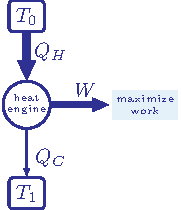
\includegraphics[width=0.4\textwidth]{graphics/chapter2/heatEngine.pdf}
        \vspace{0.5cm}
        \caption{A heat engine attempts to maximize the work done $W = Q_H - Q_C$, while transferring energy in the form of heat between two reservoirs at temperatures $T_0$ and $T_1$, respectively.}
        \label{fig: heatEngine}
    \end{subfigure}
    \\
    \vspace{2cm}
    \begin{subfigure}{0.9\textwidth}
        \centering
        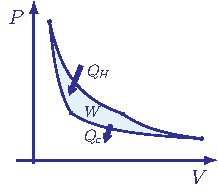
\includegraphics[width=0.5\textwidth]{graphics/chapter2/heatPathway.pdf}
        \vspace{0.5cm}
        \caption{The pathway followed by the heat engine while performing work $W$ is illustrated in the physical $P-V$ space of the system.}
        \label{fig: heatPathway}
    \end{subfigure}
    \vspace{0.5cm}
    \caption{Thermodynamics studied the pathways traversed by heat engines in the $P-V$ space which maximized the work done by it. The efficiency of such heat engines was calculated as $\eta = \frac{W}{Q_H} = \frac{Q_H - Q_C}{Q_H} = 1 - \frac{Q_C}{Q_H}$ which can be shown t be equivalent to $\eta = 1 - \frac{T_1}{T_0}$. therefore, increasing the temperature gradient in the system increased the work done by the heat engine under ideal conditions.}
    \label{fig: heatCycles}
\end{figure}
\newpage

\section{Mathematical Formulation}\label{math_form}

The first step to make the search more realistic is to assign the chemical potentials to the vertices and add constraints which allow only thermodynamically favorable reactions in the returned pathway. 
Chemical potentials are real-valued numbers. 
Hence, the inclusion of customized linear constraints and objective functions involving floating-point variables for the chemical potentials and concentrations of molecules requires us to extend the existing ILP model in M{\O}D to one using MILP incorporating these variables. This is the key focus of the current work.

MILP attempts to model the system with linear inequalities involving some variables (both integer-values and floats, hence mixed) describing the system. An infeasible system of inequalities indicates that there is no solution to the problem under those specific constraints. When a feasible solution space exists, one often attempts to optimize the solution, by maximizing (or minimizing) the value of some objective function. Tn this section, we develop the structure of the MILP model, first with using logical constraints using implications in the next section on the constraint-based model, and later, in in the discussion on implementing them, we linearize it into an MILP that can be solved using a solver.

\begin{figure}[!t]
    \centering
    \vspace{1cm}
    \begin{subfigure}{0.9\textwidth}
        \centering
        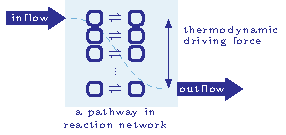
\includegraphics[width=0.75\textwidth]{graphics/chapter2/thermPathway.pdf}
        \vspace{0.5cm}
        \caption{A pathway in a chemical reaction network is a sequence of reactions that convert the source molecules (with supplied inflow) to the target molecules (with required inflow). In a thermodynamically consistent modeling, the pathway would aim to maximize the thermodynamic driving force along the pathway producing the target molecules.}
        \label{fig: thermPathway}
    \end{subfigure}
    \\
    \vspace{2cm}
    \begin{subfigure}{0.9\textwidth}
        \centering
        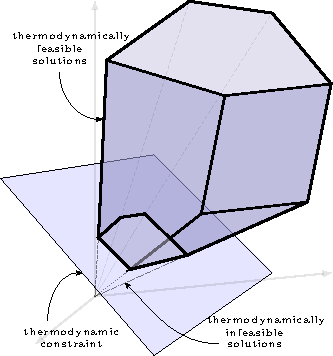
\includegraphics[width=0.55\textwidth]{graphics/chapter2/thermConstraints.pdf}
        \vspace{0.5cm}
        \caption{The addition of constraints describing the thermodynamics of the system prunes the solution space of the system, leading to hyperflow solutions that were valid earlier being thermodynamically infeasible.}
        \label{fig: thermConstraints}
    \end{subfigure}
    \vspace{0.5cm}
    \caption{A thermodynamically informed modeling of pathways in reaction networks requires the addition of constraints based on thermodynamics to capture the energetics in the system. This leads to the modification of the solution space.}
    \label{fig: thermModeling}
\end{figure}

\subsection{Constraint-Based Model}
\label{milp_implication}

\begin{figure}[!t]
    \centering
    \begin{subfigure}{0.4\textwidth}
        \centering
        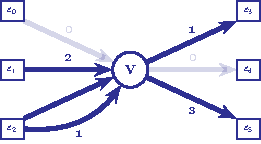
\includegraphics[width=\textwidth]{graphics/chapter2/flowConv1.pdf}
        \caption{}
        \label{fig: flowConv1}
    \end{subfigure}%
    \hfill
    \begin{subfigure}{0.4\textwidth}
        \centering
        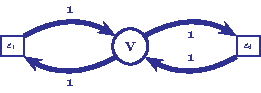
\includegraphics[width=\textwidth]{graphics/chapter2/flowConv4.pdf}
        \caption{}
        \label{fig: flowConv2}
    \end{subfigure}
    \\
    \vspace{1cm}
    \begin{subfigure}{0.4\textwidth}
        \centering
        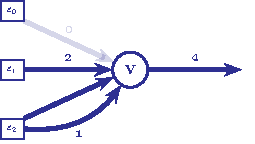
\includegraphics[width=\textwidth]{graphics/chapter2/flowConv2.pdf}
        \caption{}
        \label{fig: flowConv3}
    \end{subfigure}%
    \hfill
    \begin{subfigure}{0.4\textwidth}
        \centering
        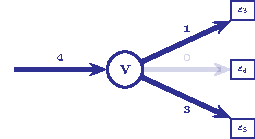
\includegraphics[width=\textwidth]{graphics/chapter2/flowConv3.pdf}
        \caption{}
        \label{fig: flowConv4}
    \end{subfigure}
    \vspace{0.2cm}
    \caption{The flow conservation constraint \ref{int_hyperflow_jakob} ensures steady-state mass conservation in the pathway. The induced hyperflow enforces that the number of copies of each vertex produced by the hyperedges equals the number of copies of the vertices used by the hyperedges. Case~\ref{fig: flowConv1} has no inflows or outflows ($v$ is neither a source vertex nor a target vertex), case~\ref{fig: flowConv2} satisfies Constraint \ref{int_hyperflow_jakob} but does not add anything physical to the pathway, case~\ref{fig: flowConv3} involves an outflow (which balances the number of copies of target vertex $v$ produced by the incident hyperedges), while case~\ref{fig: flowConv4} involves an inflow (where the number of copies of source vertex $v$ supplied is used by the out-going hyperedges).}
    \label{fig: flowConv}
\end{figure}

Since we are extending the existing integer hyperflow formulation defined earlier, the base ILP formulation for modeling flow conservation in pathways in reaction networks stated by Equation~\eqref{int_hyperflow_jakob} 
\[
\forall v\in V\colon \sum_{ e\in \overline{E} } s_{ve}^+ f_e - \sum_{ e\in \overline{E} } s_{ve}^- f_e = 0
\]

is inherited from that work. The working of Constraint~\eqref{int_hyperflow_jakob} is illustrated in the four example cases in Figure~\ref{fig: flowConv}. 

Any set of integer flow values on $E$ induces some overall reaction, which corresponds to flow values on $E^+ \cup E^-$ that make Equation~\eqref{int_hyperflow_jakob} hold.
However, the set of available source molecules is often constrained by practical considerations such as cost, ease of availability and purity.
Similarly, for the flow to be of practical utility, we could be interested in flows which maximize the outflow of a particular molecule, produce minimum side-products, and perhaps limit the use of particularly expensive reactions.
As explained while defining hyperflows, such conditions are modeled as constraints on the flow values $f_e$, in particular for $e$ in $E^+$ and $E^-$, but potentially also in $E$.
These constraints constitute a structural specification of the pathway searched for:
\begin{align}
    \text{Structural specification constraints on $f_e$ for } e \in \overline{E} \label{inflow_outflow_constraints}
\end{align}

To also incorporate thermodynamics into the modeling, we propose assigning a chemical potentials for each vertex $v$, $x^{G^0}_v$, under standard physical conditions,
which are calculated using a thermodynamic oracle described later in Chapter~\ref{ch:casestudy1}.
The differences in the chemical potentials of the target set and the source set in a reaction $e$, $x^{\Delta G}_e$, serve as the thermodynamic force driving the reaction, dictating the direction of flow of matter along that hyperedge.
In the linear regime, not far away from the equilibrium, the thermodynamic flows on a particular hyperedge is directly proportional to the thermodynamic force driving it.
The difference in chemical potential for a reaction can be manipulated by altering the concentrations of the molecules involved. 
We choose to represent the log concentration of a molecule $v$ by the variable $x_v^K$.
The nudged difference in chemical potentials for a reaction $e$ is represented as the variable, $x^{\Delta G}_e$ after taking into account the effect of the log concentration, $x_v^K$, of the molecules involved in the reaction $e$.
We would like to have an assignment of variables $x_v^K$ (within practical limits) such that the pathway consists of reactions with only negative differences in chemical potentials, of in other words, thermodynamically favorable reactions. The variables in the MILP formulation are listed in Table \ref{tab: MILPvariables}. 

\begin{table}[!t]
    \centering
    \begin{footnotesize}
    \begin{tabular}{clll}
        \\\toprule
        MILP variable & datatype & & description \\
        \midrule
        $f_e$ & integer & & flow variable for a hyperedge $e$ \\
        &&&  non-negative \\
        $x^{\Delta G}_e$ & float & & differences in chemical potential \\
        & & &  of in-vertices and out-vertices of a hyperedge $e$ \\
        & & & after accounting for their concentrations \\ 
        $x_v^K$ & float & & log concentration of a vertex $v$\\
        $t_v$ & integer & & topological ordering number \\
        &&& for vertex $v$, non-negative\\
        \midrule
        $x^{G^0}_v$ & float & & chemical potential of a vertex $v$ \\
        &&& under standard physical conditions \\
        & & & as assigned by the thermodynamic oracle \\
        $x^{\Delta G^0}_e$ & float & & differences in chemical potential \\
        &&& of in-vertices and out-vertices of a hyperedge $e$ \\
        & & & under standard physical conditions \\
        \bottomrule\\
    \end{tabular}
    \end{footnotesize}
    \caption{Variables used in the proposed constraint based formulation of pathways in a reaction network. These variables are used to formulate implication constraints in Section~\ref{milp_implication} which would be later linearized using additional auxiliary variables.}
    \label{tab: MILPvariables}
\end{table}

\begin{figure}[!h]
	\centering
	\vspace{1.5cm}
    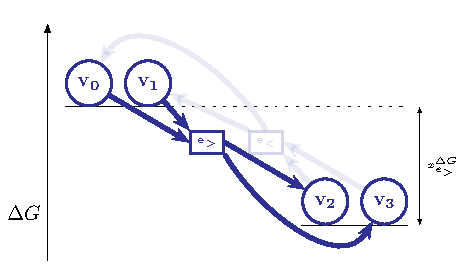
\includegraphics[width=0.75\textwidth]{graphics/chapter2/thermoConstraint.pdf}
    \vspace{0.5cm}
    \caption{Separate hyperedges have been added for the reaction $e_> : v_0 + v_1 \rightarrow v_2 + v_2$ and its reverse $e_< : v_2 + v_2 \rightarrow v_0 + v_1$. The difference in chemical potential for the hyperedge is calculated as $x_{e_>}^{\Delta G} = \Delta G(\text{RHS}) - \Delta G(\text{LHS}) = \left[\Delta G(v_2) + \Delta G(v_3)\right] - \left[\Delta G(v_0) + \Delta G(v_-)\right] = -x_{e_<}^{\Delta G}$. As a result of constraints~\ref{proposed_constraint2} and \ref{proposed_constraint3}, it is allowed to have a positive hyperflow only on the hyperedge corresponding to $e_>$. The hyperedge corresponding to $e_<$ might be assigned a hyperflow only when $x_{e_<}^{\Delta G} \leq 0$, by some possible assignment of the concentration variables $x_v^K$ of the vertices involved. Therefore, thermodynamic free energy differences dicatate the direction of mass flows in the network.}
    \label{fig: thermoConstraint}
\end{figure}

The flow $f_e$ through a hyperedge $e$ must be positive. 
\begin{equation}
    \forall e \in \overline{E}\colon  0 \leq f_e
    \label{proposed_constraint2}
\end{equation}
Since the reactions are reversible, separate hyperedges are added for the forward and backward directions.
Under specific physical conditions, thermodynamic forces dictates that either the forward or the backward direction of a reversible reaction is more likely. This is illustrated in Figure~\ref{fig: thermoConstraint}.
The direction of the flow is in the direction in which the difference in chemical potential for a hyperedge $e$, $x^{\Delta G}_e$, is negative.
The following implication-based constraint ensures that the pathway returned by the MILP solver consists of thermodynamically favorable reactions only.
\begin{equation}
    \forall e \in E\colon  f_e > 0 \implies x^{\Delta G}_e \leq 0 \label{proposed_constraint3}
\end{equation}
The difference in chemical potential, $x^{\Delta G}_e$ under arbitrary log concentration values, $x^K_v$ of the molecules participating in the reaction $e$ is calculated from the difference in chemical potential under standard conditions, $x^{G^0}_v$, by the following equations.
\begin{align}
    \forall e&\equiv (e^-, e^+) \in E\colon  \nonumber\\
    x^{\Delta G}_e &= \left(\sum_{v\in e^+} x^{G^0}_v - \sum_{v\in e^-} x^{G^0}_v\right) \nonumber\\
    &+ RT\cdot \left(\sum_{v\in e^+} x^K_v - \sum_{v\in e^-} x^K_v\right) \label{proposed_constraint4}
\end{align}
The molecules on the left side and right side of an elementary reaction belong to $e^-$ and $e^+$ respectively.
$R$ is the universal gas constant (in appropriate units) while $T$ is the absolute temperate of the system.
In a well-stirred system, $RT$ is a constant for the system.  
The log concentration of the molecules, $x_v^K$, is allowed to vary within a range $\left[x^K_v\right]_{\text{min}} \leq x_v^K \leq  \left[x^K_v\right]_{\text{max}}$,
set by practical and physical constraints detailed in Chapter \ref{ch:casestudy1}, to mimic the conditions inside a reactor.
\begin{equation}
    \left[x^K_v\right]_{\text{min}} \leq x^K_v \leq \left[x^K_v\right]_{\text{max}} \label{proposed_constraint8}
\end{equation}

\begin{figure}[!t]
    \centering
    \begin{subfigure}{\textwidth}
        \centering
        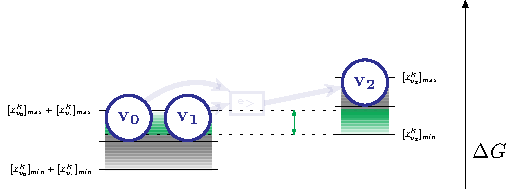
\includegraphics[width=0.75\textwidth]{graphics/chapter2/concTweak1.pdf}
        \vspace{0.4cm}
        \caption{with default values of $x_v^K$.}
        \label{fig: concTweak1}
    \end{subfigure}
    \\
    \vspace{0.8cm}
    \begin{subfigure}{\textwidth}
        \centering
        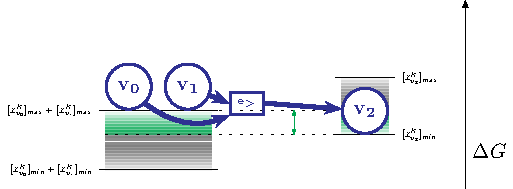
\includegraphics[width=0.75\textwidth]{graphics/chapter2/concTweak2.pdf}
        \vspace{0.4cm}
        \caption{after tweaking values of $x_v^K$}
        \label{fig: concTweak2}
    \end{subfigure}
    \vspace{0.5cm}
    \caption{Often hyperedges with assigned $x^{\Delta G^0}_e > 0$ (which are thermodynamically not feasible under standard physical conditions) can be made thermodynamically feasible by tweaking the concentration variables $x_v^K$ of the vertices involved. The hyperedge from Figure~\ref{fig: concTweak1} by raising the concentrations of vertices $v_0$ and $v_1$ and lowering the concentration of the vertex $v_2$ as shown in Figure~\ref{fig: concTweak2}.}
    \label{fig: concTweak}
\end{figure}

The control over the concentration of the molecules in the system is used in several practical scenarios to influence the equilibrium in the system.
Often, the concentration of certain molecules in the system are monitored and actively allowed to vary only within certain controlled ranges to facilitate (or inhibit) the formation of certain molecules in the system. 
The variation in the concentration of the molecules allows the model to be closer to reality, because stable molecules would have a higher concentration, while reactive intermediate molecules would be expected to have lower concentrations.
The variation in the concentration of the molecules can also make a reaction, that was thermodynamically infeasible under standard physical conditions, thermodynamically feasible under certain ranges of the concentration of the molecules involved as shown in Figure~\ref{fig: concTweak}. This then allows the corresponding hyperedge to have a non-negative flow, and be included in a pathway.

Note that the dependence of difference in the chemical potentials for a reaction $e$ on the concentrations of the molecules involved is not linear.
\begin{align*}
    x^{\Delta G}_e &= x^{\Delta G^0}_e + RT \ln\left(\frac{\prod_{v\in e^+} \text{conc}(v)}{\prod_{v\in e^-} \text{conc}(v)}\right) \\
    &= x^{\Delta G^0}_e + \frac{RT}{\ln 10}\left(\log\left(\prod_{v\in e^+} \text{conc}(v)\right)\right.\\
    & \text{\hspace{3cm}}- \left.\log\left(\prod_{v\in e^-} \text{conc}(v)\right)\right) \\
    &= x^{\Delta G^0}_e + \frac{RT}{\ln 10}\left(\sum_{v\in e^+} \log \text{conc}(v)\right.\\
    & \text{\hspace{3cm}}- \left.\sum_{v\in e^-} \log \text{conc}(v)\right)
\end{align*}
\begin{align*}
    & \text{ where, }\\
    x^{\Delta G^0}_e &= \sum_{v\in e^+} x^{G^0}_v - \sum_{v\in e^-} x^{G^0}_v
\end{align*}
However, it can be represented as a linear expression, if one chooses to represent the log concentrations of the corresponding molecule $v$, $\log_{10} \text{conc}(v)$, as a variable $x_v^K$, in the linear program. 


\subsection{Objective Function}

Formulating the search for pathways in reaction networks as an MILP problem,
allows us to add an implication constraint to rule out pathways containing one or more individual reactions not favored by thermodynamics.
However, it also enables us to exploit another feature of MILPs,
namely the objective function to quantify how likely is the entire pathway to occur.

We would like to formulate the search for pathways as an optimization problem aimed at maximizing the outflow of the target molecule(s).
To maximize the intended objective, we attempt to maximize the net thermodynamic force driving the flow.
Considering the net thermodynamic forces driving the flow to be the sum of the thermodynamic driving force for each individual reaction in the pathway,
we choose as objective function the minimization of the cumulative sum of the difference in chemical potentials for each constituent reaction with a non-zero flow. 
\begin{equation}
    \max \left(- \sum_{e\colon f_e > 0} x^{\Delta G}_e \right)
    \label{objective function}
\end{equation}
This choice of the objective function~\eqref{objective function} is a heuristic which fits  well with the cost of perturbing the system so that queried flow is effected with all reactions being thermodynamically driven in the required direction. 
Objective function~\eqref{objective function} can be related to optimal control principles and considered as the minimum work required to be done to enforce the hyperflow $f: \{e | f_e > 0\}$. Once the system is in equilibrium, it has to be slightly perturbed out of that equilibrium to sustain the hyperflow $f$.
The minimal work required to be performed to achieve the required perturbation should satisfy
\begin{equation*}
	\langle W_{\text{min}} \rangle \geq \sum_{e\colon f_e > 0} x^{\Delta G}_e
\end{equation*}
This is similar to the Crooks fluctuation theorem~\cite{crooks,crooks2} and its implication, the Jarzynski inequality~\cite{jarzynski,jarzynski2,jarzynski3}.\footnote{Equation (2) in~\cite{jarzynski} and equations (3.2) and (3.4a) in~\cite{jarzynski2} have a similar form involving the free energy on the right-hand side.}
All in all, ranking pathways by the objective function~\eqref{objective function} corresponds closely to selecting the pathway that requires the least thermodynamic work to sustain the outflow of the queried target molecule. Maximizing objective function~\eqref{objective function} becomes equivalent to minimizing the work done to perturb the system from equilibrium to achieve the desired hyperflow. 

The motivation behind choosing this particular objective function can also be argued for from the perspective of maximizing the probability of the pathway.
We interpret the free energy difference to be the measure of the probability of the reaction as
\begin{equation}
    p(e) \sim \exp\left(-x^{\Delta G}_e\right)
    \label{prob_transition}
\end{equation}
This probability for a reaction $e$ can also be argued for using the principle of local detailed balance between the rates of the reaction and its reverse where \footnote{Markovian trajectories might be coarse-grained into pathways (sets of reactions with positive hyperflow) under dilute limit, Markovian kinetics, and weak coupling between reactions.}
\begin{equation*}
    \frac{k_+(e)}{k_-(e)} = \exp\left(-\frac{x^{\Delta G}_e}{k_B T}\right)
\end{equation*}
For a Markovian process describing the sequence of reaction events along the pathway, the probability of observing the specific trajectory over time satisfies
\begin{align*}
    p\left(\bigwedge_{e\colon f_e > 0} e\right) &= \prod_{e: f_e > 0} p(e) \\
    &\sim \prod_{e\colon f_e > 0} \exp\left(-x^{\Delta G}_e\right) \\
    &= \exp\left(- \sum_{e: f_e > 0} x^{\Delta G}_e\right)
\end{align*}
Thus, for paths biased in the direction of the pathway (compared to the reverse direction), $-x^{\Delta G}_e$ accumulates additively in the exponent for the probablity.
Since, $\forall (x, y)\colon  x\leq y \iff \exp(x) \leq \exp(y)$,
maximizing the probability of the pathway is equivalent to maximizing the objective function~\eqref{objective function}.
\begin{equation*}
    \text{max} \log \left[p\left(\bigwedge_{e\colon f_e > 0} e\right)\right] \equiv \text{max} - \sum_{e: f_e > 0} x^{\Delta G}_e
    \label{log_prob}
\end{equation*}
Therefore, in the low-noise, steady-state, weak-coupling limit, maximizing the log-probability of sustaining a pathway with the hyperedges with assigned positive hyperflows decomposes approximately as maximizing a sum of negative of reaction-wise free-energy differences. The RHS of this expression~\eqref{log_prob} is the negation of the action associated with producing the desired hyperflow which is correspondingly minimized. The additivity of the objective function can be justified by the convexity of the rate function for perturbations in chemical reaction networks given by the Wentzell-Freidlin theory.~\cite{convex_rate_law}

A third way to motivate objective function~\eqref{objective function} is to use the driving force for reactions. For a reaction $e$, the thermodynamic driving force is the negative of the Gibbs free energy difference~\cite{driving_force} or $-x^{\Delta G}_e$ (which is closely related to the affinity of reactions~\cite{affinity} and positive for spontaneous reactions). The net driving force along a hyperflow would be $- \sum_{e\colon f_e > 0} x^{\Delta G}_e$ (as all hyperflows are positive, the net force adds up). Therefore, the objective corresponds to selecting pathways that are most strongly thermodynamically driven, hence most robust to perturbations.  

All in all, the objective is defensible as a heuristic, and can be motivated by a physical interpretation—but only under fairly explicit assumptions, rather than a strict consequence of the laws of thermodynamics. It should be seen more as a ranking functional, rather than a dynamical law.

\section{Implementation}
\label{milp_implement}

The objective function is a conditional sum for a set of MILP variables.
The value of the variable $x^{\Delta G}_e$ contributes to the objective function only if the corresponding hyperedge is used in the pathway.
It needs to be converted into a simple linear sum of a set of MILP variables before the MILP solver can evaluate it.  
Additionally, some constraints such as \eqref{proposed_constraint3} and \eqref{prevent_back_edges} in the mathematical formulation of the problem have been specified as implications. 
Also they need to be linearized before fed into the MILP solver.
This section describes these implementation details for the formulated MILP model in the previous section.

\subsection{Implementing the Objective function}

The objective function minimizes the cumulative sum of the differences in chemical potentials along the pathway,
$\min\left(\sum_{e\colon f_e > 0} x^{\Delta G}_e \right)$,
rather than the simple sum of differences in chemical potentials.
For all reactions $e$, $\min\left(\sum_{e \in E} x^{\Delta G}_e \right)$, in the reaction network. 
For each hyperedge $e$, a binary variable $z_e \in \{0, 1\}$ is introduced,
indicating whether that hyperedge is used in the pathway, by the following constraints
\begin{align}
    z_e = 0 &\iff f_e = 0 \label{biimp3} \\
    z_e = 1 &\iff f_e > 0 \label{biimp4}
\end{align}
We define an additional variable $\overline{x}^{\Delta G}_e$ for each hyperedge.

The assignment of the variables $\overline{x}^{\Delta G}_e$ is done by the following constraints
\begin{align}
    \overline{x}^{\Delta G}_e = 0 &\iff z_e = 0 \label{biimp1} \\
    \overline{x}^{\Delta G}_e = x^{\Delta G}_e &\iff z_e = 1 \label{biimp2}
\end{align}
The objective function is defined as the sum of these $|E|$ variables for all hyperedges in the hypergraph;
$\min\left(\sum_{e \in E} \overline{x}^{\Delta G}_e \right)$.
Hyperedges that are not utilized by the pathway have $\overline{x}^{\Delta G}_e = 0$ and would not contribute to the value of the objective function, implementing the objective function as a linear expression.


\subsection{Linearizing the Constraints}

The bi-implication constraints, Equations~\eqref{biimp3} and \eqref{biimp4}, associating the boolean variable $z_e$ to the edges $e$ is implemented using the big-M method ~\cite{bigM},
where $M > 0$ is a large positive integer constant% dont remove comment, escapes newline
\footnote{The constant $M$ has to be larger than the possible values of the variables in the MILP formulation which include the flows $f_e$ for the hyperedges and the chemical potentials $x^{G^0}_v$ for the vertices (in atomic units). In our present implementation $M = 100$ suffices.}
\begin{align}
    \forall e \in E\colon & \nonumber \\
    z_e &\leq f_e \label{linear_constraint6}\\
    M\cdot z_e &\geq f_e \label{linear_constraint7}
\end{align}
The expansion of how the added linear constraints in Equations~\eqref{linear_constraint6} and \eqref{linear_constraint7}
lead to assignment of $z_e$ satisfying the implication constraints in Equations~\eqref{biimp3} and \eqref{biimp4}
is shown in Table~\ref{tab: truth_table_constraint1}.
\begin{table}[!t]
    \centering
    \begin{footnotesize}
    \begin{tabular}{cccc}
        \\\toprule
        case of $f_e$ & \eqref{linear_constraint6} & \eqref{linear_constraint7} & implication for $z_e$ \\
        \midrule
        $f_e = 0$ & $z_e \leq 0$ & $M\cdot z_e \geq 0$ & $z_e = 0$ \\
        $f_e = k > 0$ & $z_e \leq k$ & $M\cdot z_e \geq k$ & $z_e = 1$ \\
        \bottomrule\\
    \end{tabular}
    \end{footnotesize}
    \caption{The linear constraints in Equations \eqref{linear_constraint6} and \eqref{linear_constraint7}
    are equivalent to the bi-implication constraints in Equations \eqref{biimp3} and \eqref{biimp4}.}
    \label{tab: truth_table_constraint1}
\end{table}

The implication constraint in Equation~\eqref{proposed_constraint3} determines if an hyperedge can be used in the flow depending on the differences in the chemical potentials for the hyperedges $x^{\Delta G}_e$.
This is linearized as
\begin{align}
    \forall e \in E\colon & \nonumber \\
    x^{\Delta G}_e + M\cdot (z_e - 1) &\leq 0 \label{linear_constraint1}
\end{align}
The equivalence of the added linear constraints in Equation~\eqref{linear_constraint1} to the implication constraint in Equation~\eqref{proposed_constraint3} is shown in Table~\ref{tab: truth_table_constraint2}.
\begin{table*}[!t]
    \centering
    \begin{footnotesize}
    \begin{tabular}{ccccc}
        \\\toprule
        case of $f_{e}$ & implication for $z_{e}$ & case of $x^{\Delta G}_e$ & \eqref{proposed_constraint3} satisfied? & \eqref{linear_constraint1} satisfied? \\
        \midrule
        $f_{e} = 0$ & $z_{e} = 0$ & $x^{\Delta G}_e > 0$ & True & True \\
        $f_{e} = 0$ & $z_{e} = 0$ & $x^{\Delta G}_e \leq 0$ & True & True \\
        $f_{e} > 0$ & $z_{e} = 1$ & $x^{\Delta G}_e > 0$ & False & False \\
        $f_{e} > 0$ & $z_{e} = 1$ & $x^{\Delta G}_e \leq 0$ & True & True \\
        \bottomrule\\
    \end{tabular}
    \end{footnotesize}
    \caption{The linear constraint in Equation~\eqref{linear_constraint1} is equivalent to the implication constraint in Equation~\eqref{proposed_constraint3}.}
    \label{tab: truth_table_constraint2}
\end{table*}

The bi-implication constraints in Equations~\eqref{biimp1} and \eqref{biimp2} assigns the variable $\overline{x}^{\Delta G}_e$ with the differences in the chemical potentials for the hyperedges for the evaluation of the objective function.
By utilizing the variables $z_e$, we implement the constraints as
\begin{align}
    \forall e \in E\colon & \nonumber \\
    x^{\Delta G}_e - \overline{x}^{\Delta G}_e &\leq M(1 - z_e) \label{linear_constraint2} \\
    x^{\Delta G}_e - \overline{x}^{\Delta G}_e &\geq -M(1 - z_e) \label{linear_constraint3} \\
    \overline{x}^{\Delta G}_e &\leq M\cdot z_e \label{linear_constraint4} \\
    \overline{x}^{\Delta G}_e &\geq -M\cdot z_e \label{linear_constraint5}
\end{align}
The expansion of how the added linear constraints in Equations~\eqref{linear_constraint2}, \eqref{linear_constraint3}, \eqref{linear_constraint4}, and \eqref{linear_constraint5} lead to desired assignment of $\overline{x}^{\Delta G}_e$ satisfying the implication constraints in Equations~\eqref{biimp1} and \eqref{biimp2} is shown in Table~\ref{tab: truth_table_constraint3}.

\begin{table*}[!t]
    \centering
    \begin{footnotesize}
    \begin{tabular}{@{}c@{\qquad}c*{4}{@{\qquad}c}l@{\qquad}c@{}}
        \toprule
        &&\multicolumn{4}{c}{Constraint on $\overline{x}^{\Delta G}_e$ by}\\
        \cmidrule{3-6}
        Case of $z_{e}$ & Case of $x^{\Delta G}_e$ &
            \eqref{linear_constraint2} & \eqref{linear_constraint3} & \eqref{linear_constraint4} & \eqref{linear_constraint5} &
        & Implication for $\overline{x}^{\Delta G}_e$ \\
        \midrule
        $z_{e} = 0$ & $x^{\Delta G}_e > 0$ & & & $\leq 0$ & $\geq 0$ && $=0$ \\
        $z_{e} = 0$ & $x^{\Delta G}_e \leq 0$ & & & $\leq 0$ & $\geq 0$ && $=0$ \\
        $z_{e} = 1$ & $x^{\Delta G}_e > 0$ &
            \multicolumn{6}{c}{
                \raisebox{0.5ex}{\rule{8.5em}{0.4pt}}
                \enspace Cannot happen \enspace
                \raisebox{0.5ex}{\rule{8.5em}{0.4pt}}
                } \\
        $z_{e} = 1$ & $x^{\Delta G}_e \leq 0$ & $\geq x^{\Delta G}_e$ & $\leq x^{\Delta G}_e$ & & && $= x^{\Delta G}_e$ \\
        \bottomrule
    \end{tabular}
    \end{footnotesize}
    \caption{The linear constraints of Equation~\eqref{linear_constraint2}, \eqref{linear_constraint3}, \eqref{linear_constraint4}, and \eqref{linear_constraint5}
    assign $\overline{x}^{\Delta G}_e$ according to the bi-implication constraints in Equations~\eqref{biimp1} and \eqref{biimp2}.
    Note that the third case cannot happen due to Equation~\eqref{proposed_constraint3},
    because $x^{\Delta G}_e > 0 \implies f_e = 0 \implies z_e = 0$.}
    \label{tab: truth_table_constraint3}
\end{table*}


\subsection{Implemented Model}\label{implemented model}

\begin{table*}[!b]
    \centering
    \begin{footnotesize}
    \begin{tabular}{clll}
        \toprule
        Constant & datatype & & description \\
        \midrule
        $M$ & integer & & a big integer used for \\
        &&& linearizing the constraints \\
        & & & (type promoted to float, if required) \\
        $x^{G^0}_v$ & float & & chemical potential of a vertex $v$ \\
        &&& under standard physical conditions \\
        & & & as assigned by the thermodynamic oracle \\
        $x^{\Delta G^0}_e$ & float & & differences in chemical potential \\
        &&& of in-vertices and out-vertices of a hyperedge $e$ \\
        & & & under standard physical conditions \\
        \bottomrule
    \end{tabular}
    \end{footnotesize}
    \caption{Constants in the proposed MILP formulation.
    The constants $M$ and $x^{G^0}_v$ are provided as input,
    while the constants $x^{\Delta G^0}_e$ are calculated based on the given $x^{G^0}_v$.
    }
    \label{tab: MILP constants}
\end{table*}%


For an overview, we here list the entire set of variables of the model in Table~\ref{tab: MILP variables} and the constants used in the model in Table~\ref{tab: MILP constants}. We also summarize the mixed integer linear program developed in the earlier sections.
This model is what is given to the MILP solver.

\begin{table*}[!t]
    \centering
    \begin{footnotesize}
    \begin{tabular}{clll}
        \toprule
        MILP variable & datatype & & description \\
        \midrule
        $f_e$ & integer & & flow variable for a hyperedge $e$ \\
        &&& non-negative \\
        $z_e$ & boolean & & indicator variable for a hyperedge $e$ \\
        & & & denoting if it is used in the flow \\
        $x^{\Delta G}_e$ & float & & differences in chemical potential \\
        & & &  of in-vertices and out-vertices of a hyperedge $e$ \\
        & & & after accounting for their concentrations \\ 
        $\overline{x}^{\Delta G}_e$ & float & & copy of $x^{\Delta G}_e$ used in the (linearized) objective function \\
        $x_v^K$ & float & & log concentration of a vertex $v$\\
        $t_v$ & integer & & topological ordering number \\
        &&& for vertex $v$, non-negative\\
        \bottomrule
    \end{tabular}
    \end{footnotesize}
    \caption{Variables in the proposed MILP formulation.}
    \label{tab: MILP variables}
\end{table*}%

The formulated MILP is:
\begin{align}
    & \min\left(\sum_{e \in E} \overline{x}^{\Delta G}_e \right) \label{obj_func_impl} \\    
    \forall v\in V\colon  & \sum_{ e\in \overline{E} } s_{ve}^+ f_e - \sum_{ e\in \overline{E} } s_{ve}^- f_e = 0 \tag{\ref{int_hyperflow_jakob}}
\end{align}
\begin{align}
    \text{Structural speci}&\text{fication constraints on $f_e$ for } e \in \overline{E} \tag{\ref{inflow_outflow_constraints}}\\
    \forall e&\equiv (e^-, e^+) \in E\colon \nonumber\\
    0 &\leq f_e  \tag{\ref{proposed_constraint2}} \\
    x^{\Delta G}_e &= \left(\sum_{v\in e^+} x^{G^0}_v - \sum_{v\in e^-} x^{G^0}_v\right) \nonumber\\
    & \hspace{0.5cm}+ RT\cdot \left(\sum_{v\in e^+} x^K_v - \sum_{v\in e^-} x^K_v\right) \tag{\ref{proposed_constraint4}} \\    
    0 &\geq x^{\Delta G}_e + M\cdot (z_e - 1) \tag{\ref{linear_constraint1}} \\
    M(1 - z_e) &\geq x^{\Delta G}_e - \overline{x}^{\Delta G}_e  \tag{\ref{linear_constraint2}} \\
    -M(1 - z_e) &\leq x^{\Delta G}_e - \overline{x}^{\Delta G}_e \tag{\ref{linear_constraint3}} \\
    M\cdot z_e &\geq \overline{x}^{\Delta G}_e \tag{\ref{linear_constraint4}} \\
    -M\cdot z_e &\leq \overline{x}^{\Delta G}_e \tag{\ref{linear_constraint5}} \\
    \forall v \in V\colon  & \nonumber\\
    0 &\leq t_v \leq |V| \tag{\ref{linear_constraint7}} \\
    \left[x^K_v\right]_{\text{min}} &\leq x^K_v \leq \left[x^K_v\right]_{\text{max}} \tag{\ref{proposed_constraint8}}\\\nonumber
\end{align}

The computational complexity of finding MILP solutions is in general NP-hard~\cite{Karp:72},
and even the restricted case of finding chemical pathways remains so~\cite{integer_hyperflow_np_hard}.
Despite this worst case complexity, modern MILP solvers efficiently handle most practically relevant instances in reasonable time.
From a thermodynamic perspective, it is often valuable to explore \emph{multiple} optimal or near-optimal solutions---however, MILP solvers generally only provide a single optimal solution.
Some solvers, e.g., IBM ILOG CPLEX, do provide a so-called solution pool facility for enumerating multiple solutions,
but there is little user-control for how it is populated, and in particular how solutions are compared for equality.

The thermodynamics module described in this contribution is implemented as an extension of the larger software package M{\O}D~\cite{jakob_software}, available at \url{http://mod.imada.sdu.dk/}.
The package offers the option of using multiple MILP solvers, currently IBM ILOG CPLEX, Gurobi, and Coin-OR CBC.
For the results presented here we have used Coin-OR CBC~\cite{cbc,cbc2}.
M{\O}D implements a MILP enumeration algorithm on top of the solver in use,
where one can specify a set of integer or binary variables to enumerate over.
This enumeration in M{\O}D proceeds as tree search algorithm over the domains of this set of variables,
with calls to the MILP solver for evaluating feasibility obtaining optimal solutions of subproblems~\cite{jakob_integer_hyperflows}.

In the MILP model presented here, there are variables with a continuous domain representing the concentrations and chemical potentials of the molecules.
We do not consider minor changes in these variables to represent a new solution, as long as the underlying flow is unchanged.
Hence, we carry out the enumeration over the variables $f_e,\forall e\in E$.
The resulting output is a list of different integral flows,
listed in the order of increasing value of the objective function \eqref{obj_func_impl}.

%************************************************
\section{Contextualizing this Method}
\label{discussions_method} %
%************************************************

In this section, we give a detailed comparison of our methods with some existing frameworks.
One of the closest is \emph{thermodynamics-based metabolic flux analysis} (TMFA) \cite{hatz_thermo_flow} which also utilizes mixed integer linear constraints.
Despite similarities in parts of the thermodynamic modeling, the problem solved is different, with some of the key differences being:
\begin{itemize}
    \item TMFA generates \emph{flux distributions} not containing thermodynamically infeasible reactions, while our method searches for \emph{explicitly specified pathways} mot containing thermodynamically unfavorable reactions. The flux vector generated by TMFA is real-valued as opposed to integer values for the flows in the pathways determined by our method. In many settings, the concept of a pathway involves an integer number of molecules participating in each reaction of the pathway, which aligns well with integer flows.
    \item TMFA uses a curated dataset of metabolites with chemical potentials determined by group contribution methods. In our case a semi-empirical method (GFN2-xTB) is used to assign chemical potentials to the molecules in the reaction network. However, it can be substituted by any suitable `oracle' that maps a molecule to its Gibbs free energy of the user choice. This provides flexibility and a wider applicability to this method.
    \item  We allow for a ranking of the enumerated results based on thermodynamics-based metrics. In terms of the linear program modeling, restricting the flow variables to integers allows us to enumerate solutions over the integral variables (i.e., to generate not just a single solution, but many).
    Additionally, we can enforce a partial ordering of the vertices in the returned integer hyperflow solutions, in order to guarantee their realizability as synthesis plans.
\end{itemize}

We now turn to a comparison with some of the other existing frameworks.
Formulating the problem as an MILP allows us to leverage the many algorithmic advances made in the field of MILP solvers.
This may be one reason why we are able to analyze larger reaction networks than those analyzed in \cite{miangolarra_non_ideal_CRN, seifert_thermodynamics_CRN_JCP, nicolis_thermodynamics_CRN} involving a smaller number of distinct molecules.
A further difference to these works is that they utilize kinetic rate equations derived from the law of mass action (reactions under kinetic control),
while our focus is on the differences in chemical potentials of the molecules in the reaction network near equilibrium (reactions under thermodynamics control).

Weighted directed graphs are utilized in \cite{synthesis_planning_CRN_thermodynamics} to model the thermodynamic phase space of a reaction network.
However, instead of a constant positive edge weight derived from the Gibbs free energy of the reaction,
we utilize the free energies themselves to allow for an analysis more directly based on thermodynamics.
Several other cheminformatics tools and automated protocols for computationally exploring reaction networks utilize reactive molecular dynamics simulations \cite{CRN_MD_tool1, CRN_MD_tool2, CRN_MD_tool3} or chemical heuristics \cite{CRN_kin_tool1, CRN_kin_tool2, CRN_kin_tool3, pickaxe_CRN_analyzer}.
However, to the best of our knowledge, there does not exist any computational framework for explicitly specifying and searching for pathways in reaction networks while simultaneously incorporating thermodynamic constraints in the present form. 

